\documentclass{article}

\usepackage{fancyhdr} % Required for custom headers
\usepackage{lastpage} % Required to determine the last page for the footer
\usepackage{amsmath}
\usepackage{amsfonts}
\usepackage{graphicx}
\usepackage[hidelinks]{hyperref}
% \usepackage{epstopdf} uncomment this line if using MiKTeX

% Margins
\topmargin=-0.45in
\evensidemargin=0in
\oddsidemargin=0in
\textwidth=6.5in
\textheight=9.0in
\headsep=0.25in 

\linespread{1.1} % Line spacing

% Set up the header and footer
\pagestyle{fancy}
\lhead{\hwAuthorName} % Top left header
\chead{\hwClass\ \hwTitle} % Top center header
\rhead{\hwStudentId} % Top right header
\lfoot{} % Bottom left footer
\cfoot{} % Bottom center footer
\rfoot{Page\ \thepage\ of~\pageref{LastPage}} % Bottom right footer
\renewcommand{\headrulewidth}{0.4pt} % Size of the header rule
\renewcommand{\footrulewidth}{0.4pt} % Size of the footer rule

\setlength{\parindent}{0pt} % Removes all indentation from paragraphs

\setcounter{secnumdepth}{0} % Removes default section numbers
\newcounter{homeworkProblemCounter} % Creates a counter to keep track of the number of problems

\newcommand{\homeworkProblemName}{}
\newenvironment{homeworkProblem}[1][Problem \arabic{homeworkProblemCounter}]{
	\stepcounter{homeworkProblemCounter} % Increase counter for number of problems
	\renewcommand{\homeworkProblemName}{#1} % Assign \homeworkProblemName the name of the problem
	\section{\homeworkProblemName} % Make a section in the document with the custom problem count
}{}

\newcommand{\homeworkSectionName}{}
	\newenvironment{homeworkSection}[1]{
	\renewcommand{\homeworkSectionName}{#1} % Assign \homeworkSectionName to the name of the section from the environment argument
	\subsection{\homeworkSectionName} % Make a subsection with the custom name of the subsection
}{}

%----------------------------------------------------------------------------------------
%	MATH OPERATOR
%----------------------------------------------------------------------------------------

\DeclareMathOperator*{\argmin}{arg\,min}
\DeclareMathOperator*{\argmax}{arg\,max}

%----------------------------------------------------------------------------------------
%	NAME AND CLASS SECTION
%----------------------------------------------------------------------------------------

\newcommand{\hwTitle}{Assignment\ \#1} % Assignment title
\newcommand{\hwDueDate}{Thursday,\ March\ 5,\ 2015} % Due date
\newcommand{\hwClass}{ENGG\ 5202} % Course/class
\newcommand{\hwAuthorName}{Kai Chen} % Your name
\newcommand{\hwStudentId}{1155070509} % Your student ID

%----------------------------------------------------------------------------------------
%	TITLE PAGE
%----------------------------------------------------------------------------------------

\title{
	\vspace{2in}
	\textmd{\textbf{\hwClass:\ \hwTitle}}\\
	\normalsize\vspace{0.1in}\small{Due\ on\ \hwDueDate}
	\vspace{3in}
}

\author{\textbf{\hwAuthorName}}
\date{} % Insert date here if you want it to appear below your name

%----------------------------------------------------------------------------------------

\begin{document}
\maketitle
\setcounter{page}{0}
\thispagestyle{empty}
\newpage

%----------------------------------------------------------------------------------------
%	PROBLEM 1
%----------------------------------------------------------------------------------------

% To have just one problem per page, simply put a \clearpage after each problem

\begin{homeworkProblem}

The likelihood of $\theta_1$
\[
	p(D_1|\theta_1) = p(x_1|\omega_1,\theta_1)p(x_2|\omega_1,\theta_1)
\]
The log-likelihood
\[
	l(\theta_1) = \log p(x_1|\omega_1,\theta_1) = \log p(x_1|\omega_1,\theta_1) + \log p(x_2|\omega_1,\theta_1)
\]
We determine $\theta_1$ by maximizing $l(\theta_1)$
\[
	\hat{\theta_1} = \argmax l(\theta_1)
\]
Let
\[
	\nabla l(\theta_1) = 0
\]
By substituting symbols with numeral values
\begin{eqnarray*}
	l(\theta_1) &=& 2\log\frac{2}{\theta_1} + \log(1-\frac{2}{\theta_1}) + \log(1-\frac{5}{\theta_1}) \\
	\nabla l(\theta_1) &=& - \frac{4}{\theta_1} + \frac{4}{\theta_1(\theta_1-2)} + \frac{10}{\theta_1(\theta_1-5)}	
\end{eqnarray*}
We get 
\[
	\theta_1=8 \quad or \quad \theta_1=2.5
\]
However, \( p(x|\omega_1)=0 \) when \( x>\theta_1 \) according to the densities form, if \( \theta_1=2.5 \), then \( D_1=\{2,5\} \) will not occur. Thus \( \theta_1=8 \).

Similarly, we can calculate \( \theta_2\approx14.2 \)

\end{homeworkProblem}

%----------------------------------------------------------------------------------------
%	PROBLEM 2
%----------------------------------------------------------------------------------------

\begin{homeworkProblem}

%--------------------------------------------

\begin{homeworkSection}{2.1} % Section within problem

Figure~\ref{fig:p2_1} shows \( p(x|\theta) \) versus \( x \) for \( \theta=1 \).

\begin{figure}[htbp]
\centering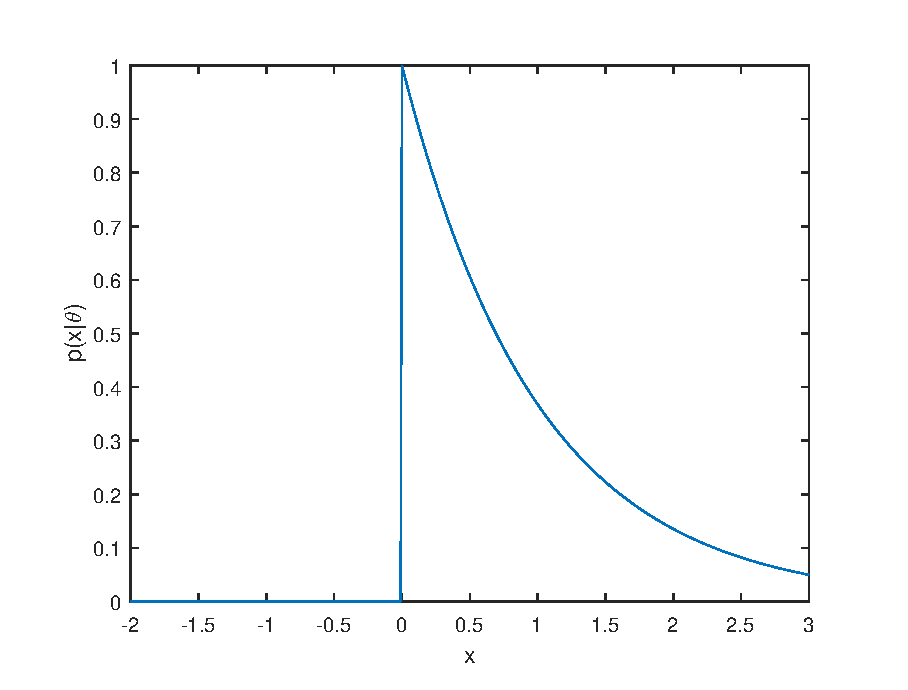
\includegraphics[width=4in]{image/p2_1}
\caption{\( p(x|\theta) \) versus \( x \) for \( \theta=1 \)}\label{fig:p2_1}
\end{figure}

Figure~\ref{fig:p2_2} shows \( p(x|\theta) \) versus \( \theta \) for \( x=2 \).

\begin{figure}[htbp]
\centering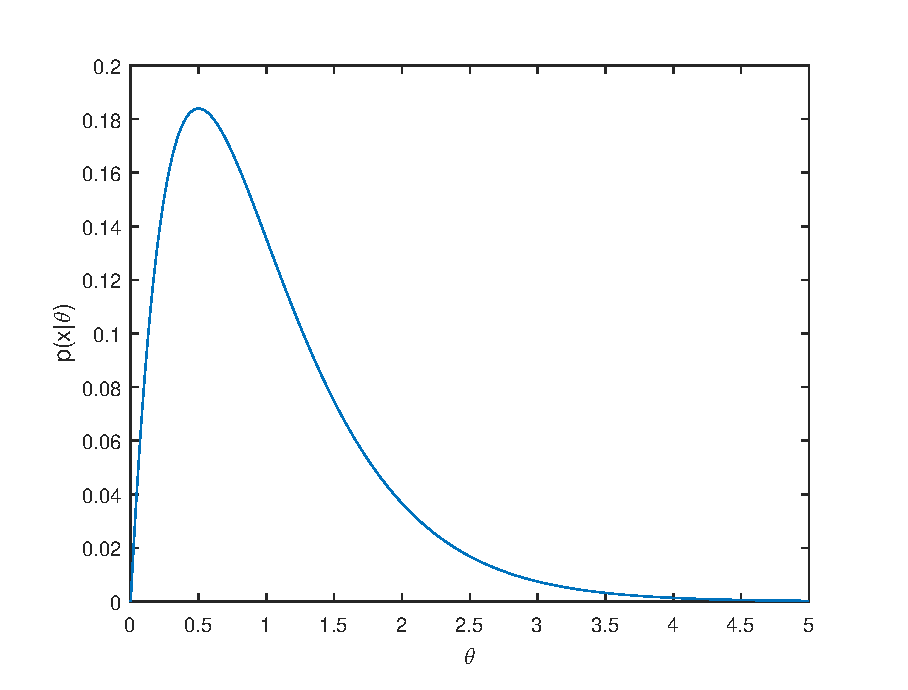
\includegraphics[width=4in]{image/p2_2}
\caption{\( p(x|\theta) \) versus \( \theta \) for \( x=2 \)}\label{fig:p2_2}
\end{figure}

\end{homeworkSection}

%--------------------------------------------

\begin{homeworkSection}{2.2}

The log-likelihood

\[
\begin{split}
	l(\theta) &= \log \prod_{k=1}^n p(x_k|\theta) \\
	&= \sum_{k=1}^n \log \theta\mathrm{e}^{-\theta x_k}
\end{split}
\]

The gradient of \( l(\theta) \)

\[
\begin{split}
	\nabla l(\theta) & = \sum_{k=1}^n \frac{(1-\theta x_k)\mathrm{e}^{-\theta x_k}}{\theta\mathrm{e}^{-\theta x_k}} \\
	&= \sum_{k=1}^n \frac{1-\theta x_k}{\theta} \\ 
	&= \frac{n-\theta \sum_{k=1}^n x_k}{\theta}
\end{split}
\]

Let \( \nabla l(\theta) = 0 \), we can calculate

\[
	\hat{\theta} = \frac{n}{\sum_{k=1}^n x_k}
\]

\end{homeworkSection}

%--------------------------------------------

\begin{homeworkSection}{2.3}

According to the law of large numbers, when \( n \) is very large, the sample average converges to the expected value.

\[
	\frac{\sum_{k=1}^n x_k}{n} \rightarrow \mathbb{E}(x) = \int_0^{\infty}\theta x\mathrm{e}^{-\theta x}\,\mathrm{d}x = \frac{1}{\theta}
\]

So \( \hat{\theta} \) approach to the true \( \theta \) when n is very large. If the samples are generated from \( p(x|\theta) \) with \( \theta=1 \), the maximum-likelihood estimate \( \hat{\theta} \) for large n is 1.

\end{homeworkSection}

\end{homeworkProblem}

\end{document}